\documentclass[
tikz,
border=5pt,
convert={density=600,
	outext=.png
}
]{standalone}


\usepackage[utf8]{inputenc}
\usepackage{stanli}
\usepackage{tikz}
\usetikzlibrary{arrows.meta,arrows,positioning,calc,backgrounds}

\begin{document}

\setcoords{-25}{30}[1][1] 
\setaxis{2} 
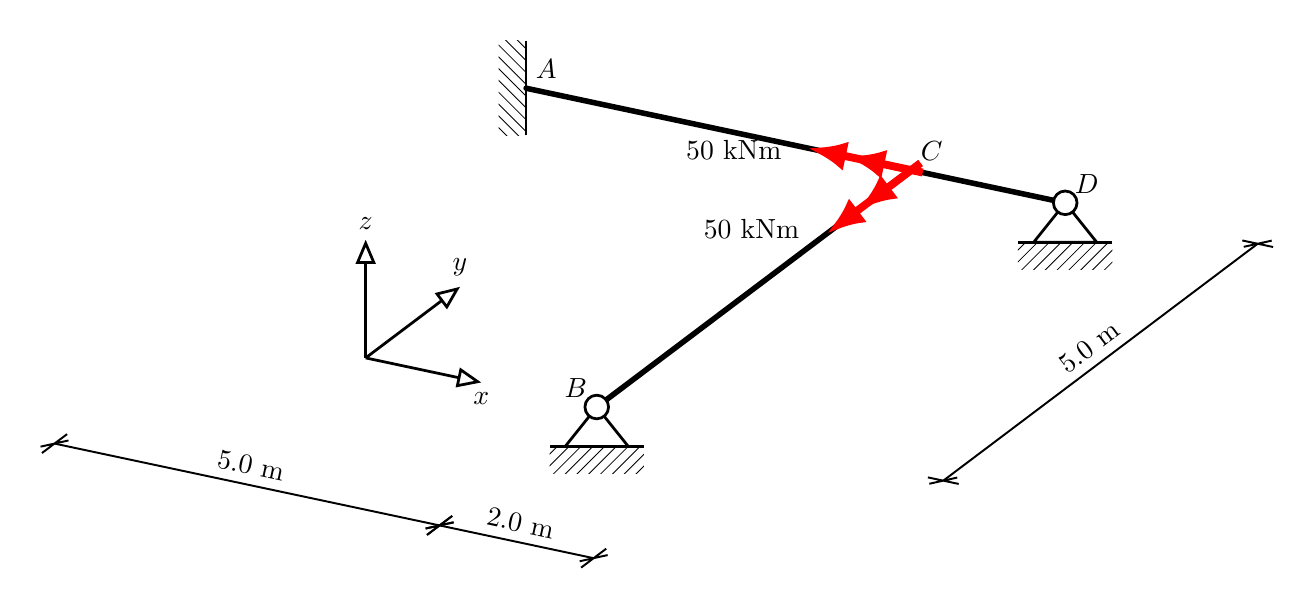
\begin{tikzpicture}[coords, background rectangle/.style={fill=white!45}, show background rectangle]

    \dpoint{a}{-5}{0}{0};
    \dpoint{b}{0}{-5}{0}; 
    \dpoint{c}{0}{0}{0};
    \dpoint{d}{2}{0}{0}; 
    \dpoint{z}{ -3.0 }{ -5.0 }{0}; 

    \daxis{1}{z}; 

    \foreach \startn/\endn in {a/c,c/d,b/c}
        \dbeam{1}{\startn}{\endn};

    \support{3}{a}[270];
    \support{1}{b}; \hinge{1}{b};
    \support{1}{d}; \hinge{1}{d};

    \begin{scope}[force/.append style={color=red,>={Latex[length=0pt 5]}},
    normalLine/.append style={line width=1mm}]
        \dload{4}{c}[90][90][ -1.5 ];
        \node[left=3mm] at ($(c)!0.25!(a)$) {$50$~kNm};

        \dload{4}{c}[90][0][ -1.5 ];
        \node[left=3mm] at ($(c)!0.25!(b)$) {$50$~kNm};
    \end{scope}

    \ddimensioning{yx}{c}{b}{2.0 + 2.5}[$5.0$~m];
    \ddimensioning{xy}{a}{c}{-5.0 - 2.5}[$5.0$~m];
    \ddimensioning{xy}{c}{d}{-5.0 - 2.5}[$2.0$~m];

    \dnotation{1}{a}{$A$}[above right];
    \dnotation{1}{b}{$B$}[above left];
    \dnotation{1}{c}{$C$}[above right];
    \dnotation{1}{d}{$D$}[above right];

\end{tikzpicture}
        
\end{document}
